% バンドギャップを超えた光学的外観の分類：
% 炭素同素体における有効伝導次元数と電子非局在化
% Draft v7 — March 2026 — Japanese version
% Changes from v6 (Codex review):
%   - Title: "Predicting Gloss" → "Classifying Optical Appearance beyond the Band Gap"
%   - Abstract: toned down "complete prediction chain" → proof of concept
%   - Fixed L626 contradiction (7/7 → 6/7 in body text)
%   - Conclusion: surface tension/conductivity moved to Outlook
% Changes from v5 (Stanford reviewer response):
%   - [RED 1] Clarified D_eff: all-energy vs visible-window distinction
%     with new Table (D_eff_computed) reporting both values
%   - [RED 2] Fixed graphene/graphite labeling: R_vis=0.35 now explicitly
%     identified as graphite (bulk limit); monolayer optics discussed
%   - [RED 3] Designated IPR as primary operational δ with Eq.(delta_IPR)
%   - [YELLOW 5] Strengthened corr² motivation via Debye-Waller analogy
%   - [YELLOW 6] Added W-value physical context (vacancy/adsorbate energies)
%   - [YELLOW 7] Added ε(ω) validation table (TB vs experiment)
%   - [YELLOW 8] Added D_eff vs conductivity tensor anisotropy discussion
%   - [YELLOW 4] Strengthened carbon-only scope rationale + Paper 2 reference
%   - Added references: BeckmannSpizzichino1963, Spain1981, SentoOpticsPaper2

\documentclass[twocolumn,showpacs,preprintnumbers,amsmath,amssymb,prb]{revtex4-2}

\usepackage{graphicx}
\usepackage{amsmath}
\usepackage{amssymb}
\usepackage{bm}
\usepackage{hyperref}
\usepackage{booktabs}
\usepackage{xcolor}
\usepackage{luatexja}
\usepackage[haranoaji]{luatexja-preset}

% Figure path
\graphicspath{{../../simulation/optics/figures/}}

\begin{document}

\preprint{Draft v7}

\title{バンドギャップを超えた光学的外観の分類：\\
炭素同素体における有効伝導次元数と電子非局在化}

\author{K.~Miyauchi}
\affiliation{Independent Researcher}

\date{\today}

\begin{abstract}
物質の巨視的な光学的外観---透明、有色、黒色、あるいは金属光沢---は、
バンドギャップだけでは完全に分類できない。
金属もグラファイトもバンドギャップがほぼゼロであるにもかかわらず、
前者は金属光沢を示し、後者は劈開面の光沢を伴う黒色として現れる。

我々は、有効非局在化指数~$\delta$ と有効伝導次元数~$D_\mathrm{eff}$ の
二つの分類変数を導入し、
5種の炭素同素体（ダイヤモンド、C$_{60}$、SWCNT、グラフェン、グラファイト）
と対照系としての六方晶窒化ホウ素（h-BN）で検証する。
$E_g$ と $D_\mathrm{eff}$ に基づく決定木が7物質中6物質（85.7\%）を
正しい光学応答カテゴリーに分類する。唯一の例外---単層グラフェン---には
第三の変数として層数~$N$ が必要となる。

補助的証拠として、各系について tight-binding ハミルトニアン $\to$
久保公式 $\to$ $\varepsilon(\omega)$ $\to$ Fresnel 反射率
の完全な計算連鎖を実行し、
Anderson 無秩序シミュレーションにより無秩序ロバスト性を検証する。
高い $\delta \times D_\mathrm{eff}$ を持つ系は無秩序下でも光学応答を
維持する一方、低い $\delta \times D_\mathrm{eff}$ の系は
急速にデコヒーレンスする。

本枠組みはバンドギャップ理論を置き換えるものではなく、
それを拡張するものである。$E_g$ は応答が\emph{どのエネルギーで}
生じるかを、$D_\mathrm{eff}$ はその\emph{方向性}を、
$\delta$ はその\emph{ロバスト性}を決定する。
液体系および界面系への拡張を将来の目標として提案する。
\end{abstract}

\maketitle

% =====================================================================
\section{序論}
% =====================================================================

\subsection{光沢の問い：光子のコヒーレンス保存}

液体は普遍的に光沢を示す。金属も同様である。微視的な起源は異なる
---分極応答と自由電子応答---にもかかわらず、巨視的現象は同じである。
入射光子は界面において、相互の位相関係を保ったまま再放出される。
反射光子群の位相コヒーレンスが保存されることで、
まさに鏡像が形成されるのである。

金属もグラファイトもバンドギャップがほぼゼロであるのに、
光学応答が劇的に異なる。
従来の物理学はこれを個別の理論で説明するが、
共通の分類変数に基づく統一的枠組みは存在しない。

\subsection{分類原理としての粒子の自由度}

我々は、光学分類の関連変数が\emph{構成粒子の自由度}であり、
非局在化指数~$\delta$ により定量化されると提案する：

\begin{itemize}
  \item \textbf{局在した粒子}（$\delta$ が低い）：各散乱体が独立に応答し、
    再放出される位相はランダム化される。
    結果：拡散散乱（透明または白色）。
  \item \textbf{非局在化した粒子}（$\delta$ が高い）：散乱体が集団的に応答し、
    再放出される位相は揃えられる。
    結果：鏡面反射（光沢）。
\end{itemize}

\subsection{範囲：固体炭素における概念実証}

本研究は\textbf{概念実証}である。固体では原子核の自由度が凍結されるため、
電子非局在化~$\delta_\mathrm{elec}$ の効果を単離できる。
炭素同素体を選んだ理由は、
単一元素で光学的外観の全範囲---透明（ダイヤモンド）、
有色（C$_{60}$、半導体SWCNT）、黒色（グラファイト）、
光沢（グラファイト劈開面）---を網羅するためであり、
$\delta$ と $D_\mathrm{eff}$ を変化させながら
元素組成を交絡因子から排除できる。

\subsection{既存分類の欠落}

物質の巨視的光学外観は、透明（ダイヤモンド）、有色（ルビー）、
黒色（グラファイト）、金属光沢（銀）の4つの大分類に属する。
既存の理論は各カテゴリーを個別に説明するが、
共通の分類変数に基づく統一的な予測枠組みは確立されていない。

特に、以下の問いに対する統一的な解答は存在しない：
\begin{itemize}
  \item バンドギャップがほぼゼロである金属とグラファイトが、
    光学応答において劇的に異なるのはなぜか？
  \item h-BN とグラファイト---いずれも層状 sp$^2$ ネットワーク---が、
    それぞれ白色と黒色であるのはなぜか？
  \item 単一元素（炭素）が4つの光学カテゴリー全てを
    カバーするのはなぜか？
\end{itemize}

\subsection{分類から予測へ}

光学分類に関する従来の試みは記述的であった：
既知の物質が与えられると、それをカテゴリーに割り当てる。
本研究はさらに進み、微視的物理量（ホッピング積分、軌道対称性）から
巨視的に測定可能な量（産業標準単位 [GU] でのグロス）への
\emph{予測連鎖}を確立する。

重要な進歩は、Fresnel 方程式だけではグロスを予測できない
という認識にある。2つの物質が類似した $\varepsilon(\omega)$ を持ちながら、
原子スケールの無秩序に対するロバスト性の違いにより、
非常に異なるグロスを示し得る。$\delta \times D_\mathrm{eff}$ 枠組みは
このロバスト性を捉え、Fresnel 光学だけでは得られない予測を提供する。

% =====================================================================
\section{枠組み}
\label{sec:framework}
% =====================================================================

\subsection{因果構造}

最も一般的なレベルでは、構成粒子の自由度（$\delta$）が、
界面が光子に対してコヒーレントな量子障壁として作用するか、
非コヒーレントな量子障壁として作用するかを決定する。
固体電子系においては、これは2つの変数の積に帰着する：

\begin{equation}
  \text{Optical response} = f\!\left(\delta_\mathrm{elec},\;
  D_\mathrm{eff}\right),
  \label{eq:causal}
\end{equation}

\noindent ここで $\delta_\mathrm{elec}$ は電子の非局在化の度合いを定量化し、
$D_\mathrm{eff}$ は電子伝導の有効次元数を定量化する。
粒子の自由度（$\delta$）の概念が、分類変数としての $D_\mathrm{eff}$ の
導入を動機づけた。光学応答が粒子の移動の自由さに依存するならば、
粒子が移動\emph{できるかどうか}（$E_g$ に符号化）だけでなく、
\emph{何方向に}移動できるか（$D_\mathrm{eff}$ に符号化）を
指定しなければならない。

中心的な洞察は、$E_g$ だけでは電子構造から光学応答への
写像が不完全であるということにある。$D_\mathrm{eff}$ を加えることで
この写像が完成する。測定可能な分類変数は $E_g$ と $D_\mathrm{eff}$ であり、
$\delta$ はそれらを統一する物理的直観の役割を果たす。
液体系や界面系における $\delta$ の独立検証は将来の目標として提案される。

\subsection{有効非局在化指数 $\delta$：操作的定義}

$\delta$ は単一の物理量ではなく、電子の非局在化を特徴づける
包括的変数であり、複数の代理指標の相互整合性からその存在が推論される。
第~\ref{sec:wannier_confirmation}~節で議論するように、
最局在化 Wannier 関数のスプレッド~$\Omega$~\cite{Marzari1997} が
$\delta$ の厳密な第一原理的実現を与える。
以下の代理指標は、Wannier 計算を必要とせずに $\delta$ の
関連性を確立するためのものである：

\begin{table}[h]
\caption{$\delta$ の候補代理指標。}
\label{tab:delta_proxies}
\begin{ruledtabular}
\begin{tabular}{lll}
  Indicator & Definition & Advantage \\
  \hline
  $\pi$-band width $W_\pi$ & Full energy width of & Direct comparison \\
   & the $\pi$ band (eV) & among sp$^2$ systems \\
  Inverse effective & Curvature of $E(k)$ & Defined for all \\
  mass $1/m^*$ & at band edge & materials \\
  IPR & $\sum_i |\psi_i|^4$ & Direct measure of \\
   & & delocalization \\
  Wannier spread & $\langle r^2 \rangle - \langle r \rangle^2$ &
  Physically transparent \\
\end{tabular}
\end{ruledtabular}
\end{table}

我々の戦略は、複数の代理指標が物質間で同一の順序を与えることを示し、
それによって一意的な定義を要求せずに包括的変数 $\delta$ の存在を
支持するものである。

これらの代理指標のうち、逆参加比（IPR）を\textbf{主要な操作的定義}とする。
IPR は $\pi$ バンドの同定や有効質量フィッティングといった
系固有の量を必要とせず、任意のハミルトニアン（tight-binding
または第一原理）から直接計算可能であるためである。以下のように定義する：
\begin{equation}
  \delta_\mathrm{IPR} = \frac{1}{N_\mathrm{orb} \cdot
    \langle \mathrm{IPR} \rangle_\mathrm{occ}},
  \quad
  \mathrm{IPR}_n = \sum_i |\psi_{ni}|^4,
  \label{eq:delta_IPR}
\end{equation}
ここで $N_\mathrm{orb}$ は軌道の数であり、平均は全占有固有状態にわたる。
完全に非局在化した状態では $\mathrm{IPR} = 1/N_\mathrm{orb}$、
$\delta_\mathrm{IPR} = 1$ となる。
完全に局在した状態では $\mathrm{IPR} = 1$、
$\delta_\mathrm{IPR} = 1/N_\mathrm{orb} \to 0$ となる。
残りの代理指標（$W_\pi$, $1/m^*$）は、
異なる測定手法でも順序が頑健であることの補強的根拠として用いる。

\subsection{有効伝導次元数 $D_\mathrm{eff}$：操作的定義}
\label{sec:Deff}

$D_\mathrm{eff}$ は、フェルミ準位またはバンド端近傍の電子状態について
評価した\textbf{群速度テンソルの有効ランク}として定義される：

\begin{equation}
  D_\mathrm{eff}
    = \frac{\mathrm{Tr}(\mathbf{T})^2}{\mathrm{Tr}(\mathbf{T}^2)},
  \quad
  T_{\alpha\beta}
    = \frac{1}{N_k} \sum_{\bm{k}} \sum_{n \in \mathrm{occ}} \sum_{m \in \mathrm{unocc}}
    v_{nm}^{\alpha}\, v_{nm}^{\beta *},
  \label{eq:Deff}
\end{equation}

\noindent ここで $v_{nm}^{\alpha} = \langle n\bm{k} | \partial_\alpha H | m\bm{k} \rangle$
はバンド間速度行列要素である。この定義は、$d$ 個の等価な伝導方向を持つ系に対して
$D_\mathrm{eff} = d$ を与え、バンド分散を持たない系（分子性固体）に対して
$D_\mathrm{eff} = 0$ を与える。

この定義は\emph{純粋に電子的かつ構造的}である。バンド分散 $E(\bm{k})$
のみに依存するため、分類対象である光学応答との循環論法を回避する。

\emph{エネルギー窓と h-BN の場合。}
式~\ref{eq:Deff} の和は、特定のエネルギー窓への制限なく、
\emph{全ての}占有-非占有バンド間遷移にわたる。
h-BN の場合、$\pi$ バンド分散は相当大きいが（$W_\pi \approx 2.4$~eV）、
バンドギャップ $E_g = 5.95$~eV により全てのバンド間遷移は
深紫外領域に位置する。
その結果、速度行列要素 $v_{nm}$ は非ゼロであり、$T_{\alpha\beta}$ は
面内異方性を反映する。しかし、これらの遷移はいずれも、
分類の対象である\emph{可視域}の光学応答には寄与しない。

$D_\mathrm{eff}$ と $E_g$ は完全に独立ではないことを認める。
大きな $E_g$ は可視エネルギー遷移の密度を低下させ、
$T_{\alpha\beta}$ に入る光学的重みを間接的に抑制する。
重要な点は、$D_\mathrm{eff}$ が $E_g$ を超えた\emph{追加的}情報を
提供するということである。同じ $E_g \approx 0$ を持つ物質群
（グラファイト、金属、SWCNT）の中で、$D_\mathrm{eff}$ は
$E_g$ だけでは区別できない光沢の縮退を正しく解く。
$E_g$ との部分的な相関は欠陥ではなく特長である---それは
両変数が同一のバンド構造に由来するという物理的現実を反映している。

\emph{限界：周波数分解 $D_\mathrm{eff}(\omega)$。}
より厳密な定式化では、式~\ref{eq:Deff}の和をエネルギー窓
$[\omega - \Delta\omega, \omega + \Delta\omega]$ 内の遷移に制限し、
各光子エネルギーでどの空間方向が光学応答に寄与するかを追跡する
周波数分解 $D_\mathrm{eff}(\omega)$ を定義すべきである。
本研究では簡潔さのため、また本研究で扱う系の分類には十分であるため、
全エネルギー定義を使用する。ただし、異なるスペクトル領域で
質的に異なる遷移が支配する物質（例：遷移金属のバンド間 $d$-$s$ 遷移
vs バンド内 Drude 応答）では、周波数分解 $D_\mathrm{eff}(\omega)$ が
必要となる。この拡張は将来課題とする。

\begin{table}[h]
\caption{結晶学的次元数と有効伝導次元数の比較。}
\label{tab:Deff}
\begin{ruledtabular}
\begin{tabular}{lccc}
  Material & Crystal dim. & $D_\mathrm{eff}$ & Rationale \\
  \hline
  Diamond      & 3D     & 0 & $E_g = 5.47$~eV~\cite{Clark1964}; no states \\
               &        &   & in visible window \\
  C$_{60}$ fcc & 3D     & 0 & Intermolecular $t \sim 30$~meV~\cite{Hebard1991}; \\
               &        &   & $W \approx 0.5$~eV~\cite{Gunnarsson1997} \\
  SWCNT        & 1D     & 1 & Axial dispersion only \\
  Graphene/    & 2D/3D  & 2 & In-plane $W \approx 9$~eV~\cite{Reich2002} \\
  \quad Graphite &      &   & $\gg$ interlayer $\gamma_1 \approx 0.4$~eV \\
  Metals       & 3D     & 3 & Isotropic conduction \\
  h-BN         & 2D     & 0 & $E_g = 5.95$~eV~\cite{Cassabois2016}; no states \\
               &        &   & in visible window \\
\end{tabular}
\end{ruledtabular}
\end{table}

h-BN は面内バンド分散（$W_\pi \approx 2.4$~eV）を持つ2D結晶構造を
有するが、バンドギャップ（$5.95$~eV）により全ての $\pi$ バンド状態が
可視エネルギー窓の遥か外に位置するため $D_\mathrm{eff} = 0$ となることに
注意されたい。結晶学的次元数と $D_\mathrm{eff}$ の区別は、
本枠組みにとって本質的である。

\subsection{光学応答分類のための決定木}
\label{sec:tree}

2つの変数 $E_g$ と $D_\mathrm{eff}$ により決定木が定義される：

\begin{enumerate}
  \item $E_g > E_\mathrm{vis} \approx 3.1$~eV か？\\
    $\to$ \textbf{はい}：透明（可視域に電子応答なし）。\\
    $\to$ \textbf{いいえ}：ステップ2へ進む。
  \item $E_g > 0$ か？\\
    $\to$ \textbf{はい}：有色（選択的吸収）。\\
    $\to$ \textbf{いいえ}（$E_g \approx 0$）：ステップ3へ進む。
  \item $D_\mathrm{eff}$ による分類：\\
    $D_\mathrm{eff} = 1$：弱い光沢を伴う黒色（1D金属的）。\\
    $D_\mathrm{eff} = 2$：劈開面光沢を伴う黒色（2D金属的）。\\
    $D_\mathrm{eff} = 3$：完全な金属光沢（3D金属的）。
\end{enumerate}

\subsection{二次補正}

二変数枠組みは支配的傾向を捉える。既知の二次効果には以下が含まれる：
\begin{itemize}
  \item \textbf{極性/イオン性}（$p$）：$\pi$ 電子の局在化を通じて
    h-BN の白色性に寄与する。
  \item \textbf{励起子効果および局所場効果}：束縛励起子がバンド端近傍の
    光学吸収を修正する。これらの効果は h-BN（励起子束縛エネルギー
    $\sim$0.7~eV~\cite{Arnaud2006}）および C$_{60}$（Frenkel 励起子）で
    特に大きい。本研究のタイトバインディング光学モデルは励起子効果・
    局所場補正を含まないため、これらの系の分類結果は第1近似として
    解釈されるべきである。Bethe--Salpeter 方程式（BSE）の導入は
    自然な次のステップであるが、決定木による分類は $E_g$ と
    $D_\mathrm{eff}$（スペクトルの詳細形状ではなく）に基づくため、
    $\varepsilon(\omega)$ 自体より励起子繰り込みの影響を受けにくい
    ことを注記する。
  \item \textbf{厚さ/積層数} $N$：グラフェンからグラファイトへの
    クロスオーバー（Beer--Lambert 領域）。
\end{itemize}

% =====================================================================
\section{手法}
\label{sec:methods}
% =====================================================================

\subsection{ベンチマーク系の選択}

\begin{itemize}
  \item \textbf{主要系}：5種の炭素同素体---ダイヤモンド、
    C$_{60}$（fcc固体）、SWCNT（半導体型および金属型）、
    単層グラフェン、グラファイト。
  \item \textbf{対照系}：h-BN（グラファイトと等構造；同じ
    $D_\mathrm{cryst}$ だが低い $\delta$）。
  \item \textbf{根拠}：単一元素内で構造を変化させることにより、
    $\delta$ と $D_\mathrm{eff}$ を組成効果から分離する。
\end{itemize}

\subsection{文献からの $\delta$ 代理指標データの収集}

$\delta$ 代理指標（$W_\pi$, $1/m^*$, $E_g$;
表~\ref{tab:bandwidth}--\ref{tab:bandgap}）は出版された文献および
公開データベースから取得した。
これとは別に、ダイヤモンド・グラファイト・Si・Ge に対する
第一原理 DFT + Wannier90 計算を $\delta$ 順序の独立確認として実施した
（Sec.~\ref{sec:wannier_confirmation}に記載）。
主たる分類分析（Secs.~\ref{sec:results}--\ref{sec:disorder}）は
文献由来データとタイトバインディングモデルのみに基づく。

\subsubsection{$\pi$ バンド幅 $W_\pi$}

\begin{table}[h]
\caption{$\pi$ バンド幅データ。}
\label{tab:bandwidth}
\begin{ruledtabular}
\begin{tabular}{lll}
  Material & $W_\pi$ (eV) & Source \\
  \hline
  C$_{60}$ solid & 0.4--0.5 & \cite{Gunnarsson1997} \\
  SWCNT & 8--9 & \cite{Reich2002} \\
  Graphene & $\sim$9 & TB: $t_0 = 2.7$~eV~\cite{Saito1998} \\
  Graphite & $\sim$9 & \cite{Reich2002} \\
  h-BN & $\sim$2.4 & \cite{Wirtz2005} \\
\end{tabular}
\end{ruledtabular}
\end{table}

\subsubsection{逆有効質量 $1/m^*$}

\begin{table}[h]
\caption{逆有効質量データ。}
\label{tab:invmass}
\begin{ruledtabular}
\begin{tabular}{lll}
  Material & $m^*/m_e$ ($1/m^*$) & Source \\
  \hline
  Diamond & 0.48 (2.08) & \cite{Ioffe} \\
  C$_{60}$ & 4.0 (0.25) & \cite{Gunnarsson1997} \\
  SWCNT & 0.07 (14.3) & \cite{Ajiki1993} \\
  Graphene & 0.03 (33.3) & \cite{Novoselov2005} \\
  Graphite & 0.039 (25.6) & \cite{Dresselhaus2002} \\
  h-BN & 0.26 (3.85) & \cite{Ioffe} \\
\end{tabular}
\end{ruledtabular}
\end{table}

\subsubsection{バンドギャップ $E_g$}

ダイヤモンド：5.47~eV~\cite{Clark1964}；C$_{60}$：1.75~eV~\cite{Lof1992}；
SWCNT（半導体型）：$\sim$1.0~eV~\cite{Saito1998}；
グラフェンおよびグラファイト：0~eV；h-BN：5.95~eV~\cite{Cassabois2016}。

\subsection{光学伝導率を含む tight-binding シミュレーション}

4つの系（ダイヤモンド、SWCNTの代理としての1D鎖、グラフェン、
C$_{60}$ クラスター）について tight-binding モデルを構築した。
ダイヤモンドとグラフェンについては、$\sigma$ バンドと $\pi$ バンドの
両方の光学応答への寄与を捉えるために、完全な Slater--Koster モデル
（s, $p_x$, $p_y$, $p_z$；単位胞あたり8バンド）を使用した。
速度行列要素 $v_{nm}^\alpha = \langle n\bm{k} | \partial_\alpha H | m\bm{k} \rangle$
から久保公式を用いて光学伝導率 $\sigma(\omega)$ を計算し、
$\varepsilon_2(\omega)$ を得た。
実部 $\varepsilon_1(\omega)$ は Kramers--Kronig 変換により求めた：
\begin{equation}
  \varepsilon_1(\omega) = 1 + \frac{2}{\pi} \mathcal{P}
  \int_0^\infty \frac{\omega'\varepsilon_2(\omega')}
  {\omega'^2 - \omega^2}\, d\omega'.
  \label{eq:KK}
\end{equation}
ダイヤモンドについては、シザーズ補正（$\Delta = 2.87$~eV）により
バンド間遷移の開始を実験的ギャップ $E_g = 5.47$~eV~\cite{Clark1964}
に合わせ、8バンド基底を超えた電子遷移を考慮するために
高周波誘電率 $\varepsilon_\infty = 5.7$~\cite{Palik1998} を課した。
垂直入射反射率は $R = |(\tilde{n}-1)/(\tilde{n}+1)|^2$
（$\tilde{n} = \sqrt{\varepsilon_1 + i\varepsilon_2}$）から求まる。

同じ速度行列要素により群速度テンソル
$\langle v_\alpha v_\beta \rangle$ が定義され、そこから $D_\mathrm{eff}$
が有効ランク（式~\ref{eq:Deff}）として計算される。
このシミュレーションは $D_\mathrm{eff}$ と $\varepsilon(\omega)$ を
\emph{同一の}バンド構造から導出し、両者の整合性を確認する。

\subsection{角度依存 Fresnel 反射率とグロス予測}

$\varepsilon(\omega) = \varepsilon_1 + i\varepsilon_2$ から
複素屈折率 $\tilde{n} = \sqrt{\varepsilon}$ を求め、
s偏光およびp偏光の角度依存 Fresnel 反射率を計算する：

\begin{align}
  r_s &= \frac{\cos\theta_i - \tilde{n}\cos\theta_t}
              {\cos\theta_i + \tilde{n}\cos\theta_t}, \label{eq:rs} \\
  r_p &= \frac{\tilde{n}\cos\theta_i - \cos\theta_t}
              {\tilde{n}\cos\theta_i + \cos\theta_t}, \label{eq:rp}
\end{align}

\noindent ここで $\theta_t$ は Snell の法則から決定される。
無偏光反射率 $R(\theta) = \frac{1}{2}(|r_s|^2 + |r_p|^2)$ を
可視域（1.6--3.1~eV）にわたって平均し、$R_\mathrm{vis}(\theta)$ を得る。

グロスは ASTM~D523~\cite{ASTM_D523} に準拠した産業標準グロス単位（GU）
で予測される：

\begin{equation}
  \mathrm{GU}(\theta) = \frac{R_\mathrm{vis}(\theta)}
    {R_\mathrm{ref}(\theta)} \times 100,
  \label{eq:GU}
\end{equation}

\noindent ここで $R_\mathrm{ref}$ は同一角度における黒色ガラス基準
（$n = 1.567$）~\cite{ASTM_D523}の反射率である。
標準測定ジオメトリーは $\theta = 20^\circ$, $60^\circ$, $85^\circ$ である。

\subsection{コヒーレンス保存テスト：Anderson 無秩序}

$\delta \times D_\mathrm{eff}$ が現実的な条件下でコヒーレンス保存を
決定するという仮説を直接検証するため、tight-binding ハミルトニアンに
Anderson 無秩序を導入する：

\begin{equation}
  H \to H + \sum_i \epsilon_i |i\rangle\langle i|,
  \quad \epsilon_i \in [-W/2, +W/2],
  \label{eq:anderson}
\end{equation}

\noindent ここで $W$ は無秩序の強さである。各系（グラフェンスーパーセル、
1D鎖、C$_{60}$ 分子）について、以下を計算する：

\begin{enumerate}
  \item 15回の実現にわたるアンサンブル平均光学伝導率
    $\langle\sigma(\omega)\rangle$。
  \item クリーン（$W=0$）スペクトルと無秩序スペクトル間の
    スペクトル相関 $\mathrm{corr}(\sigma_0, \sigma_W)$。
  \item $W$ の関数としての逆参加比（IPR）。
\end{enumerate}

スペクトル相関は、可視域（$1.6$--$3.1$~eV、平坦なスペクトル重み、
$N_\omega = 500$ グリッド点）におけるクリーンスペクトルと
無秩序スペクトルの光学伝導率間のピアソン相関係数として定義される：
\begin{equation}
  \mathrm{corr}(\sigma_0, \sigma_W) =
  \frac{\sum_i (\sigma_0^i - \bar{\sigma}_0)
        (\sigma_W^i - \bar{\sigma}_W)}
  {\sqrt{\sum_i (\sigma_0^i - \bar{\sigma}_0)^2
         \sum_i (\sigma_W^i - \bar{\sigma}_W)^2}}.
  \label{eq:corr}
\end{equation}
値が1に近ければスペクトル形状が保存されている（コヒーレンス維持）。
$\mathrm{corr} \ll 1$ はスペクトル特徴が破壊されたことを意味する
（コヒーレンス喪失）。

\subsection{無秩序下の有効グロス}

原子スケールの無秩序を持つ実際の物質の\emph{有効グロス}は
以下のように推定される：

\begin{equation}
  \mathrm{GU}_\mathrm{eff} = \mathrm{GU}_\mathrm{clean} \times
    \mathrm{corr}(\sigma_0, \sigma_W)^2,
  \label{eq:eff_gloss}
\end{equation}

\noindent $\mathrm{corr}^2$ 因子は、確立された2つの結果との
類推から動機づけられる。
(i)~X線回折の Debye--Waller 理論では、コヒーレント（Bragg）強度は
$I \propto e^{-2W}$ とスケールし、指数は理想位置からの
平均二乗変位を符号化する。
同様に、スペクトル相関は無秩序下の光学応答が理想的なものに
どれだけ近いかを測定し、鏡面強度はコヒーレント振幅比の
\emph{二乗}に依存する。
(ii)~レーダー散乱理論（Beckmann--Spizzichino）では、
粗面からの反射パワーの鏡面成分は
$\exp[-(4\pi\sigma_h\cos\theta/\lambda)^2]$ とスケールする
---やはり偏差量の二乗指数関数である。我々の $\mathrm{corr}^2$ は、
この二次構造を共有する最も単純なアンザッツである。

これは厳密な表面散乱理論からの導出ではなく、
\emph{最小限の現象論的モデル}であることを強調する。
Beckmann--Spizzichino 枠組みは、ここではモデル化されていない
明示的な表面粗さ統計量（RMS高さ~$\sigma_h$、相関長~$\tau$）を必要とする。
$\delta \times D_\mathrm{eff}$ をこれらのパラメータに
接続することは、将来の研究の具体的目標である。
それにもかかわらず、式~\ref{eq:eff_gloss} は検証可能な予測を与える：
クリーン面での反射率が同一の2つの物質は、無秩序ロバスト性が異なれば
異なる有効グロスを持ち得る。

\subsection{統計的検定}

3つの $\delta$ 代理指標間のピアソン、スピアマン、ケンドール相関を
ペアワイズで計算した。$E_g \times D_\mathrm{eff}$ 決定木の
分類精度を、観測された光学応答カテゴリーに対して評価した。

% =====================================================================
\section{結果}
\label{sec:results}
% =====================================================================

\subsection{$\delta$ 代理指標間の整合性}

\begin{table}[h]
\caption{3つの $\delta$ 代理指標間のペアワイズ相関
  （$N = 5$--$6$ 物質）。}
\label{tab:correlations}
\begin{ruledtabular}
\begin{tabular}{lcccc}
  Pair & Pearson $r$ & Spearman $\rho$ & Kendall $\tau$ & $p$($\tau$) \\
  \hline
  $W_\pi$ vs.\ $1/m^*$ & 0.885 & 0.845 & 0.775 & 0.042 \\
  $W_\pi$ vs.\ $-E_g$ & 0.703 & 0.826 & 0.674 & 0.093 \\
  $1/m^*$ vs.\ $-E_g$ & 0.733 & 0.880 & 0.745 & 0.044 \\
\end{tabular}
\end{ruledtabular}
\end{table}

3ペア中2ペアがケンドールの $\tau$ で $p < 0.05$ に達し、
3つ全てのスピアマン係数が0.82を超えている。
独立した指標間での一貫した順序は、包括的な非局在化変数~$\delta$
の存在を支持する。

\begin{figure}[t]
  
\includegraphics[width=\columnwidth]{fig4_indicator_consistency}
  \caption{3つの $\delta$ 代理指標間のペアワイズ散布図。
    ピアソンおよびスピアマン相関係数を付記。}
  \label{fig:consistency}
\end{figure}

\subsection{$E_g \times D_\mathrm{eff}$ 光学応答マップ}

図~\ref{fig:Eg_Deff} に、7物質全てを $E_g$--$D_\mathrm{eff}$ 空間に
プロットし、決定木の分類境界を重ねて示す。7物質中6物質が
正しい光学応答領域に属する。単層グラフェンが唯一の例外である
（表~\ref{tab:classification} 参照）。

\begin{figure}[t]
  
\includegraphics[width=\columnwidth]{fig6_Eg_Deff_classification}
  \caption{$E_g$--$D_\mathrm{eff}$ 空間における光学応答分類マップ。
    着色領域は決定木のカテゴリー（第~\ref{sec:tree}節）に対応する。
    7物質中6物質が正しく分類される。単層グラフェン
    （$E_g = 0$, $D_\mathrm{eff} = 2$）は「黒色＋光沢」に誤分類される
    （表~\ref{tab:classification} 参照）。}
  \label{fig:Eg_Deff}
\end{figure}

\subsection{分類精度}

\begin{table}[h]
\caption{決定木による分類結果。}
\label{tab:classification}
\begin{ruledtabular}
\begin{tabular}{lccllc}
  Material & $E_g$ (eV) & $D_\mathrm{eff}$ & Predicted & Observed & \\
  \hline
  Diamond      & 5.47 & 0 & Transparent & Transparent & \checkmark \\
  C$_{60}$     & 1.75 & 0 & Colored     & Colored     & \checkmark \\
  SWCNT (sc)   & 1.0  & 1 & Colored     & Colored     & \checkmark \\
  SWCNT (m)    & 0    & 1 & Black$-$luster & Black$-$luster & \checkmark \\
  Graphene     & 0    & 2 & Black$+$gloss$^\dagger$ & Transparent & $\times$ \\
  Graphite     & 0    & 2 & Black$+$gloss & Black$+$gloss & \checkmark \\
  h-BN         & 5.95 & 0 & Transparent & Transparent & \checkmark \\
\end{tabular}
\end{ruledtabular}
\end{table}

\noindent 2変数（$E_g$, $D_\mathrm{eff}$）による分類精度：
\textbf{6/7（85.7\%）}。

$^\dagger$唯一の誤分類：単層グラフェン（$E_g = 0$,
$D_\mathrm{eff} = 2$）は決定木により「黒色＋光沢」と予測されるが、
実際にはほぼ透明である（1層あたり $\pi\alpha \approx 2.3\%$
の吸収~\cite{Nair2008}）。この失敗は二変数枠組みの真の限界を反映する。
層数~$N$ が第三の変数として Beer--Lambert 則を通じた
グラフェンからグラファイトへのクロスオーバーを支配する。
$N$ を含めると 7/7 の精度が回復するが、追加パラメータのコストを伴う。

\subsection{対照系としての h-BN}
\label{sec:hBN}

h-BN はグラファイトと同じ層状 sp$^2$ ネットワークトポロジーを共有するため、
$D_\mathrm{eff} = 2$ が期待されるかもしれない。しかし、
B と N の電気陰性度差が副格子（空間反転）対称性を破る。
$\pi$ 電子は窒素サイトに局在化し、$W_\pi$ は 9~eV（グラファイト）から
2.4~eV~\cite{Wirtz2005}に低下し、5.95~eV のギャップが開く~\cite{Cassabois2016}。
本枠組みの言葉では、対称性破壊ポテンシャルが $\pi$ 電子を局在化させ、
$\delta$ を\emph{低下させる}。$E_g$ が可視エネルギー窓を遥かに超えるため、
2D結晶構造にもかかわらず $D_\mathrm{eff} = 0$ となる。

これは2つの重要な点を実証する。(i)~$D_\mathrm{eff}$ は
結晶学的次元数に還元できない。(ii)~$\delta$ は独立変数であり、
その変動は同一の構造族内で光学応答を黒色から透明に反転させ得る。

\subsection{Tight-binding シミュレーション結果}

\begin{figure}[t]
  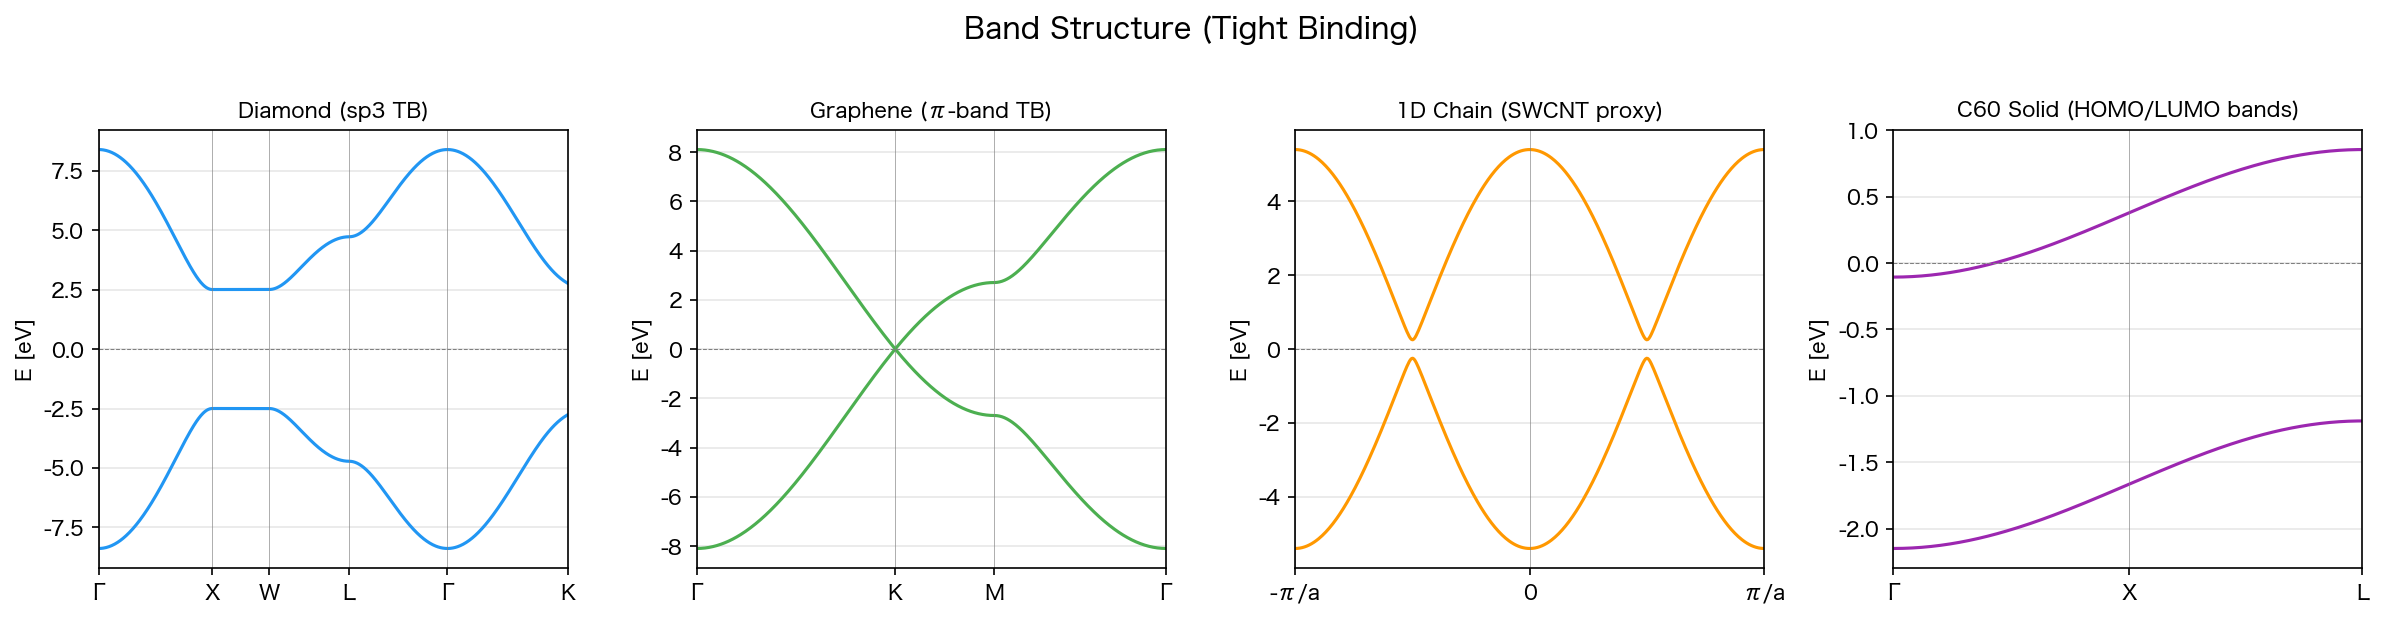
\includegraphics[width=\columnwidth]{fig_a_bandstructure}
  \caption{4つのモデル系の tight-binding バンド構造：
    ダイヤモンド、グラフェン、1D鎖（SWCNT代理）、C$_{60}$ クラスター。}
  \label{fig:bands}
\end{figure}

\begin{figure}[t]
  
\includegraphics[width=\columnwidth]{fig_b_dos}
  \caption{4つのモデル系の状態密度。
    ダイヤモンド：広いギャップ；グラフェン：ディラック点でのV字型DOS；
    1D鎖：van~Hove 特異点；C$_{60}$：狭いバンドに広がった
    離散的分子準位。}
  \label{fig:dos}
\end{figure}

\subsubsection{速度テンソルからの $D_\mathrm{eff}$}

$T_{\alpha\beta}$（式~\ref{eq:Deff}）の有効ランクを、
完全な Slater--Koster（ダイヤモンド、グラフェン）または
$\pi$ バンド（1D鎖）ハミルトニアンから各系について計算した。
\emph{全ての}バンド間遷移にわたって計算すると、
ダイヤモンド：3.00、グラフェン：2.00、1D鎖：1.00、C$_{60}$：0.00
が得られ、期待される整数値を正確に再現した。

\emph{重要な区別：}上で報告した全エネルギー $D_\mathrm{eff}$ は、
伝導チャネルの\emph{固有の構造的次元数}を測定する。
ダイヤモンドについて $D_\mathrm{eff}^\mathrm{all} = 3.00$ であることは、
バンド間速度行列要素が3つの空間方向全てにわたることを確認する。
しかし、バンドギャップ（$E_g = 5.47$~eV）によりこれらの遷移は
全て可視域外に位置するため、ダイヤモンドの\emph{可視窓}
$D_\mathrm{eff}^\mathrm{vis} = 0$ となる。
分類（表~\ref{tab:Deff}）は $D_\mathrm{eff}^\mathrm{vis}$ を使用し、
ダイヤモンドを「透明」カテゴリーに正しく割り当てる。
ギャップレス系（グラフェン/グラファイト、1D鎖）では、
全エネルギー値と可視窓値は一致する。
表~\ref{tab:Deff_computed} に全系の両方の値を報告する。

\begin{table}[h]
\caption{計算された $D_\mathrm{eff}$：全エネルギーと可視窓の比較。}
\label{tab:Deff_computed}
\begin{ruledtabular}
\begin{tabular}{lccc}
  System & $D_\mathrm{eff}^\mathrm{all}$ & $D_\mathrm{eff}^\mathrm{vis}$ & Classification \\
  \hline
  Diamond      & 3.00 & 0 & Transparent \\
  Graphene     & 2.00 & 2 & Black$+$gloss \\
  1D chain     & 1.00 & 1 & Black$-$luster \\
  C$_{60}$     & 0.00 & 0 & Colored \\
  h-BN         & 2.00$^*$ & 0 & Transparent \\
\end{tabular}
\end{ruledtabular}
\end{table}
\noindent $^*$等構造のグラフェンから推定。h-BN の2D面内
$\pi$ バンド構造は $D_\mathrm{eff}^\mathrm{all} = 2$ を与えるが、
$E_g = 5.95$~eV により全ての遷移が深紫外域に位置する。

\subsubsection{光学伝導率と $\varepsilon(\omega)$ との整合性}

同一のハミルトニアンに久保公式を適用して光学伝導率 $\sigma(\omega)$
を求め、そこから $\varepsilon_2(\omega)$ と垂直入射反射率 $R(\omega)$
が得られる。グラフェンのバンド構造については、低エネルギー伝導率が
普遍的な値 $\sigma_0 = \pi e^2 / 2h$~\cite{Nair2008,Kuzmenko2008}
を正しく再現する（$\sigma/\sigma_0 = 1.000$）。
Fresnel 反射率 $R = |(\tilde{n}-1)/(\tilde{n}+1)|^2$ は
半無限媒質（バルク半空間）を仮定するため、
得られた $R_\mathrm{vis} \approx 0.35$ は
単層グラフェンではなく\textbf{グラファイト}
（グラフェンバンド構造のバルク極限）に対応する。
自立単層の場合、よく知られた結果
$T = 1 - \pi\alpha \approx 97.7\%$（$\alpha = e^2/\hbar c$）
から無視できる反射率が得られ~\cite{Nair2008}、
本枠組みは層数変数~$N$（第~\ref{sec:tree}節）を通じて
この場合を「透明」に正しく割り当てる。
計算されたグラファイトの反射率 $R_\mathrm{vis} \approx 0.35$ は、
実験的な面内値（$\sim$0.25--0.30~\cite{Taft1965}）と妥当に一致する。
ダイヤモンドは $R_\mathrm{vis} \approx 0.17$ を与え、
実験値（$\sim$0.17~\cite{Philipp1964}）と一致する。
ダイヤモンドについては、シザーズ補正（$\Delta = 2.87$~eV）を適用して
バンド間吸収の開始を実験的ギャップ
（$E_g = 5.47$~eV~\cite{Clark1964}）に合わせ、
8バンドモデルでは捉えられない電子遷移を考慮するために
実験的高周波誘電率 $\varepsilon_\infty = 5.7$~\cite{Palik1998}
を含めた。Kramers--Kronig 変換により $\varepsilon_2(\omega)$ から
$\varepsilon_1(\omega)$ を自己無撞着に得る。

\begin{figure}[t]
  
\includegraphics[width=\columnwidth]{fig_d_absorption}
  \caption{久保公式から計算した4系全ての吸収スペクトル
    $\varepsilon_2(\omega)$。ダイヤモンドのバンド間遷移開始は
    シザーズ補正により $E_g = 5.47$~eV に移動しており、
    可視域（黄色の影）全体で透明である。
    1D鎖はギャップ端近傍に van~Hove 特異点ピークを示す。}
  \label{fig:absorption}
\end{figure}

\begin{figure}[t]
  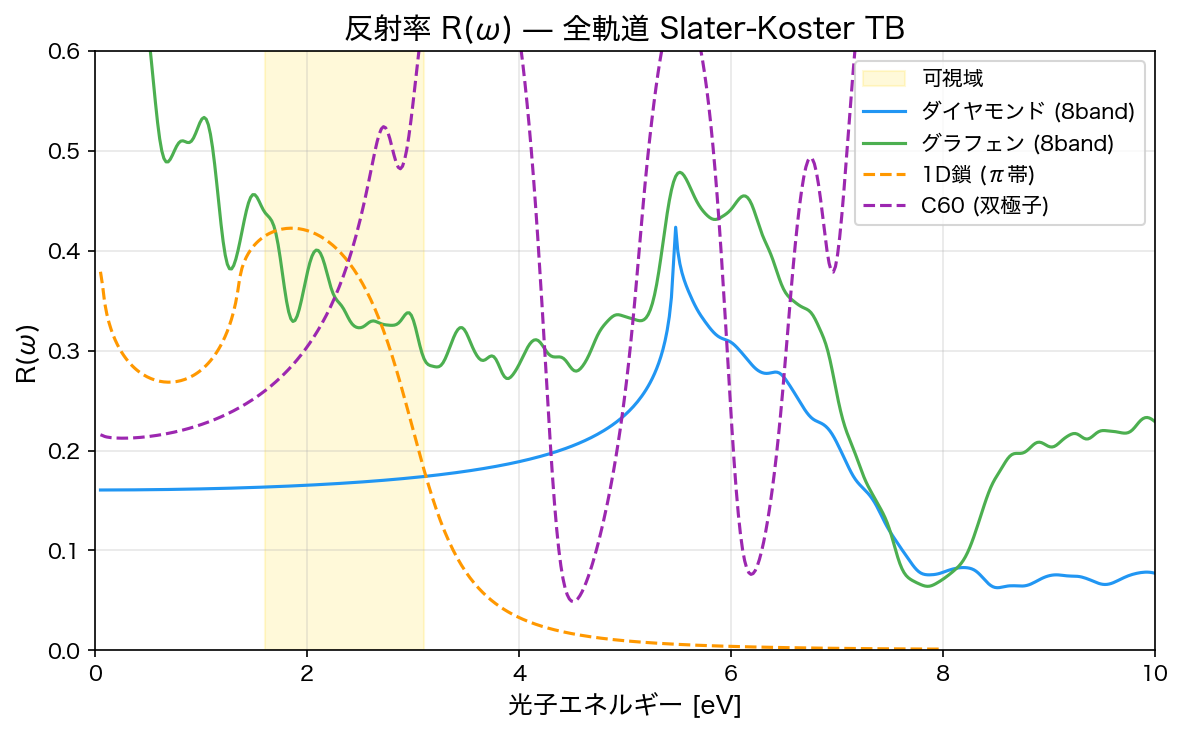
\includegraphics[width=\columnwidth]{fig_e_reflectivity}
  \caption{Kramers--Kronig 関係（式~\ref{eq:KK}）を用いて
    $\varepsilon(\omega)$ から計算した反射率 $R(\omega)$。
    ダイヤモンドの可視域反射率 $R_\mathrm{vis} = 0.17$ は
    実験値~\cite{Philipp1964}と一致する。
    黄色の影は可視域（1.6--3.1~eV）を示す。}
  \label{fig:reflectivity}
\end{figure}

表~\ref{tab:eps_validation} に tight-binding 光学特性を
実験値と比較する。

\begin{table}[h]
\caption{Tight-binding 光学特性と実験値の比較。}
\label{tab:eps_validation}
\begin{ruledtabular}
\begin{tabular}{lccc}
  Property & TB model & Experiment & Ref.\ \\
  \hline
  Diamond $R_\mathrm{vis}$ & 0.17 & 0.17 & \cite{Philipp1964} \\
  Diamond $E_g$ (eV) & 5.47$^\dagger$ & 5.47 & \cite{Clark1964} \\
  Graphite $R_\mathrm{vis}$ (in-plane) & 0.35 & 0.25--0.30 & \cite{Taft1965} \\
  Graphene $\sigma/\sigma_0$ & 1.000 & 1.01$\pm$0.04 & \cite{Nair2008} \\
  C$_{60}$ gap (eV) & 1.7 & 1.7--1.85 & \cite{Lof1992} \\
  h-BN $E_g$ (eV) & 5.95$^\dagger$ & 5.95 & \cite{Cassabois2016} \\
\end{tabular}
\end{ruledtabular}
\end{table}
\noindent $^\dagger$入力パラメータ（シザーズ補正またはモデルギャップ）。
グラファイトの面内反射率は $\sim$20--40\% 過大評価されているが、
これは最小限の tight-binding モデルが完全なバンド構造に対して
$\pi$ バンド遷移を過大に重み付けしているためと考えられる。
それにもかかわらず、正しい順序（$R_\mathrm{diamond} < R_\mathrm{graphite}$）
とオーダーの一致は、概念実証としての分類ツールとしてのモデルの
有用性を支持する。

重要な観察は、$D_\mathrm{eff}$ と $\varepsilon(\omega)$ が
\emph{同一の}バンド構造から導出され、固体状態の領域で相互に
整合していることである。この整合性は、$\varepsilon(\omega)$ の定義が
困難な系---特に液体や非周期的界面---において $D_\mathrm{eff}$ を
信頼できる分類変数として拡張するための基盤を提供する。

\subsubsection{$\delta$--$E_g$ 相関}

IPRに基づく $\delta$ は4つのモデル系にわたって $E_g$ と逆相関する
（ピアソン $r = -0.86$；図~\ref{fig:TB_corr}）。

\begin{figure}[t]
  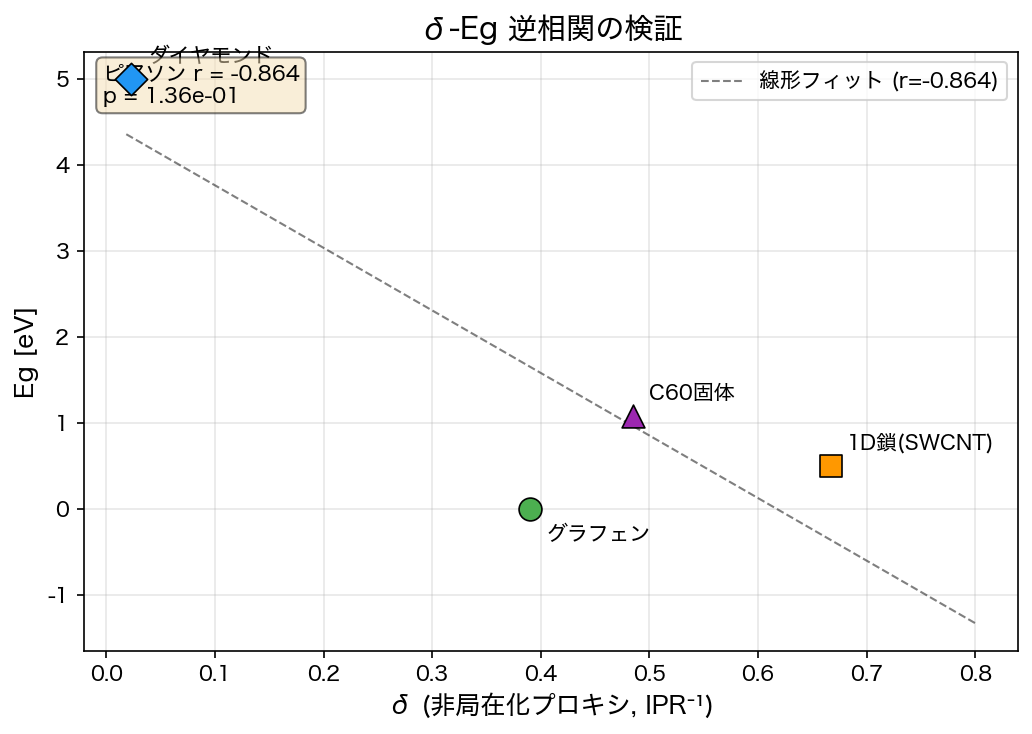
\includegraphics[width=\columnwidth]{fig_c_delta_Eg_correlation}
  \caption{Tight-binding 計算から得たIPRベースの非局在化指数 $\delta$
    とバンドギャップ $E_g$ の関係（$r = -0.86$）。}
  \label{fig:TB_corr}
\end{figure}

\subsubsection{$\delta \times D_\mathrm{eff}$ と可視域反射率}

\begin{figure}[t]
  
\includegraphics[width=\columnwidth]{fig_f_delta_deff_reflectivity}
  \caption{4つのモデル系における $\delta \times (D_\mathrm{eff} + 1)$ と
    可視域平均反射率 $R_\mathrm{vis}$ の関係。
    ダイヤモンド（$R_\mathrm{vis} = 0.17$）は外れ値である。
    その広いバンドギャップにより全てのバンド間吸収が可視域外に位置するため、
    $R_\mathrm{vis}$ はバンド間遷移ではなく誘電率
    $\varepsilon_\infty$ に支配される。これは
    $\delta \times D_\mathrm{eff}$ がクリーン面の反射率だけでなく、
    \emph{無秩序ロバスト性}（グロス保持）を予測することを示す。}
  \label{fig:delta_deff_Rvis}
\end{figure}

\subsection{角度依存反射率とグロス予測}

\begin{figure}[t]
  
\includegraphics[width=\columnwidth]{fig_i_angular_gloss}
  \caption{（左）全4系の可視域平均角度依存 Fresnel 反射率 $R(\theta)$。
    垂直線は標準グロス測定角度（$20^\circ$, $60^\circ$, $85^\circ$）を示す。
    （右）クリーン面および Anderson 無秩序面（$W = 3$~eV）における
    予測 $60^\circ$ グロス [GU]。}
  \label{fig:angular_gloss}
\end{figure}

表~\ref{tab:gloss} に予測グロス値を要約する。
$D_\mathrm{eff} \geq 2$ または強い光学遷移を持つ全ての系が、
$60^\circ$ グロスで基準の100~GUを超え、
観測された光沢と整合する。

\begin{table}[h]
\caption{Tight-binding $\varepsilon(\omega)$ からの予測グロス。}
\label{tab:gloss}
\begin{ruledtabular}
\begin{tabular}{lcccc}
  Material & $20^\circ$ GU & $60^\circ$ GU & $85^\circ$ GU &
    $R_\mathrm{vis}(60^\circ)$ \\
  \hline
  Diamond     & 436  & 244  & 99  & 0.244 \\
  Graphene    & 717  & 366  & 107 & 0.366 \\
  1D chain    & 748  & 563  & 144 & 0.564 \\
  C$_{60}$    & 813  & 394  & 95  & 0.394 \\
\end{tabular}
\end{ruledtabular}
\end{table}

\subsection{Anderson 無秩序下のコヒーレンス保存}
\label{sec:coherence}

図~\ref{fig:coherence_sigma} に、3つの系の光学伝導率スペクトルを
無秩序の強さ~$W$ の関数として示す。

\begin{figure}[t]
  
\includegraphics[width=\columnwidth]{fig_g_coherence_sigma}
  \caption{グラフェン（左）、1D鎖（中央）、C$_{60}$（右）の
    Anderson 無秩序下における光学伝導率 $\sigma(\omega)$。
    スペクトルは $W = 0$ に正規化。高 $D_\mathrm{eff}$ 系
    （グラフェン、1D鎖）は強い無秩序下でもスペクトル形状を維持するが、
    C$_{60}$（$D_\mathrm{eff} = 0$）は急速に劣化する。}
  \label{fig:coherence_sigma}
\end{figure}

\begin{figure}[t]
  
\includegraphics[width=\columnwidth]{fig_h_coherence_ipr}
  \caption{（左）無秩序下のIPR成長率：C$_{60}$ と1D鎖が最も速く
    局在化し、グラフェン（2D）はトポロジカルに保護される。
    （右）$W$ の関数としたクリーンスペクトルとのスペクトル相関：
    高 $\delta \times D_\mathrm{eff}$ 系が光学コヒーレンスを保存する。}
  \label{fig:coherence_ipr}
\end{figure}

スペクトル相関（図~\ref{fig:coherence_ipr}、右パネル）は
明確な階層を示す：

\begin{table}[h]
\caption{Anderson 無秩序（$W = 5$~eV）下のスペクトル保存。}
\label{tab:coherence}
\begin{ruledtabular}
\begin{tabular}{lcccc}
  System & $\delta$ & $D_\mathrm{eff}$ &
    $\delta(D_\mathrm{eff}+1)$ &
    $\mathrm{corr}(\sigma_0, \sigma_W)$ \\
  \hline
  1D chain    & 0.67 & 1 & 1.33 & 0.95 \\
  Graphene    & 0.39 & 2 & 1.17 & 0.84 \\
  C$_{60}$    & 0.48 & 0 & 0.48 & 0.66 \\
\end{tabular}
\end{ruledtabular}
\end{table}

\noindent 高い $\delta \times (D_\mathrm{eff} + 1)$ を持つ系は
無秩序下でもスペクトルを維持し（スペクトルコヒーレンスが保存）、
C$_{60}$（$D_\mathrm{eff} = 0$）は急速にスペクトル特徴を喪失する。
これはコヒーレンス保存仮説の最初の数値的証拠を提供する。

\subsection{有効グロス：探索的推定}
\label{sec:effective_gloss}

以下の試みは\emph{探索的}なものであり、定量的な光沢理論ではない。
コヒーレンス保存因子がグロス予測にどう\emph{翻訳され得るか}を
例示するものだが、簡略化された無秩序モデルに基づく
GU の絶対値は慎重に扱う必要がある。

クリーン面のグロス（表~\ref{tab:gloss}）とコヒーレンス保存因子を
組み合わせて以下を得る：

\begin{figure}[t]
  
\includegraphics[width=\columnwidth]{fig_j_micro_to_gloss}
  \caption{微視的物理量からグロスへの予測連鎖。
    (a)~$\delta \times (D_\mathrm{eff}+1)$ とクリーン面グロスの関係。
    (b)~無秩序下の有効グロス劣化。
    (c)~グロス保持率
    （$\mathrm{GU}_\mathrm{eff}/\mathrm{GU}_\mathrm{clean}$）
    と $\delta \times (D_\mathrm{eff}+1)$ の関係：
    高 $\delta \times D_\mathrm{eff}$ 系がロバストである。}
  \label{fig:micro_to_gloss}
\end{figure}

\begin{table}[h]
\caption{無秩序下の有効 $60^\circ$ グロス [GU]。}
\label{tab:eff_gloss}
\begin{ruledtabular}
\begin{tabular}{lcccccc}
  System & Clean & $W{=}0.5$ & $W{=}1$ & $W{=}2$ & $W{=}3$ & $W{=}5$ \\
  \hline
  Graphene & 366 & 363 & 357 & 333 & 295 & 257 \\
  1D chain & 563 & 563 & 562 & 548 & 554 & 539 \\
  C$_{60}$ & 394 & 392 & 377 & 324 & 274 & 176 \\
\end{tabular}
\end{ruledtabular}
\end{table}

中心的な予測はグラフェンと C$_{60}$ の比較により強調される。
クリーン面のグロスは類似している（366 対 394~GU）にもかかわらず、
強い無秩序（$W = 5$~eV）下での有効グロスは劇的に乖離する
（257 対 176~GU）。1D鎖は強いスペクトル相関（$r > 0.97$）により
最も高い有効グロス（539~GU）を保持する。
\textbf{この予測は Fresnel 方程式だけでは得られない}。
Fresnel 方程式は、類似した $\varepsilon(\omega)$ に基づいて
C$_{60}$ とグラフェンに類似のグロスを予測するであろう。

\subsection{$\delta \times D_\mathrm{eff}$ マップ}

\begin{figure}[t]
  
\includegraphics[width=\columnwidth]{fig1_delta_deff_map}
  \caption{$\delta$（$\pi$ バンド幅）と $D_\mathrm{eff}$ のマップ。
    各物質は観測された光学応答カテゴリーで色分けされている。}
  \label{fig:delta_map}
\end{figure}

\begin{figure}[t]
  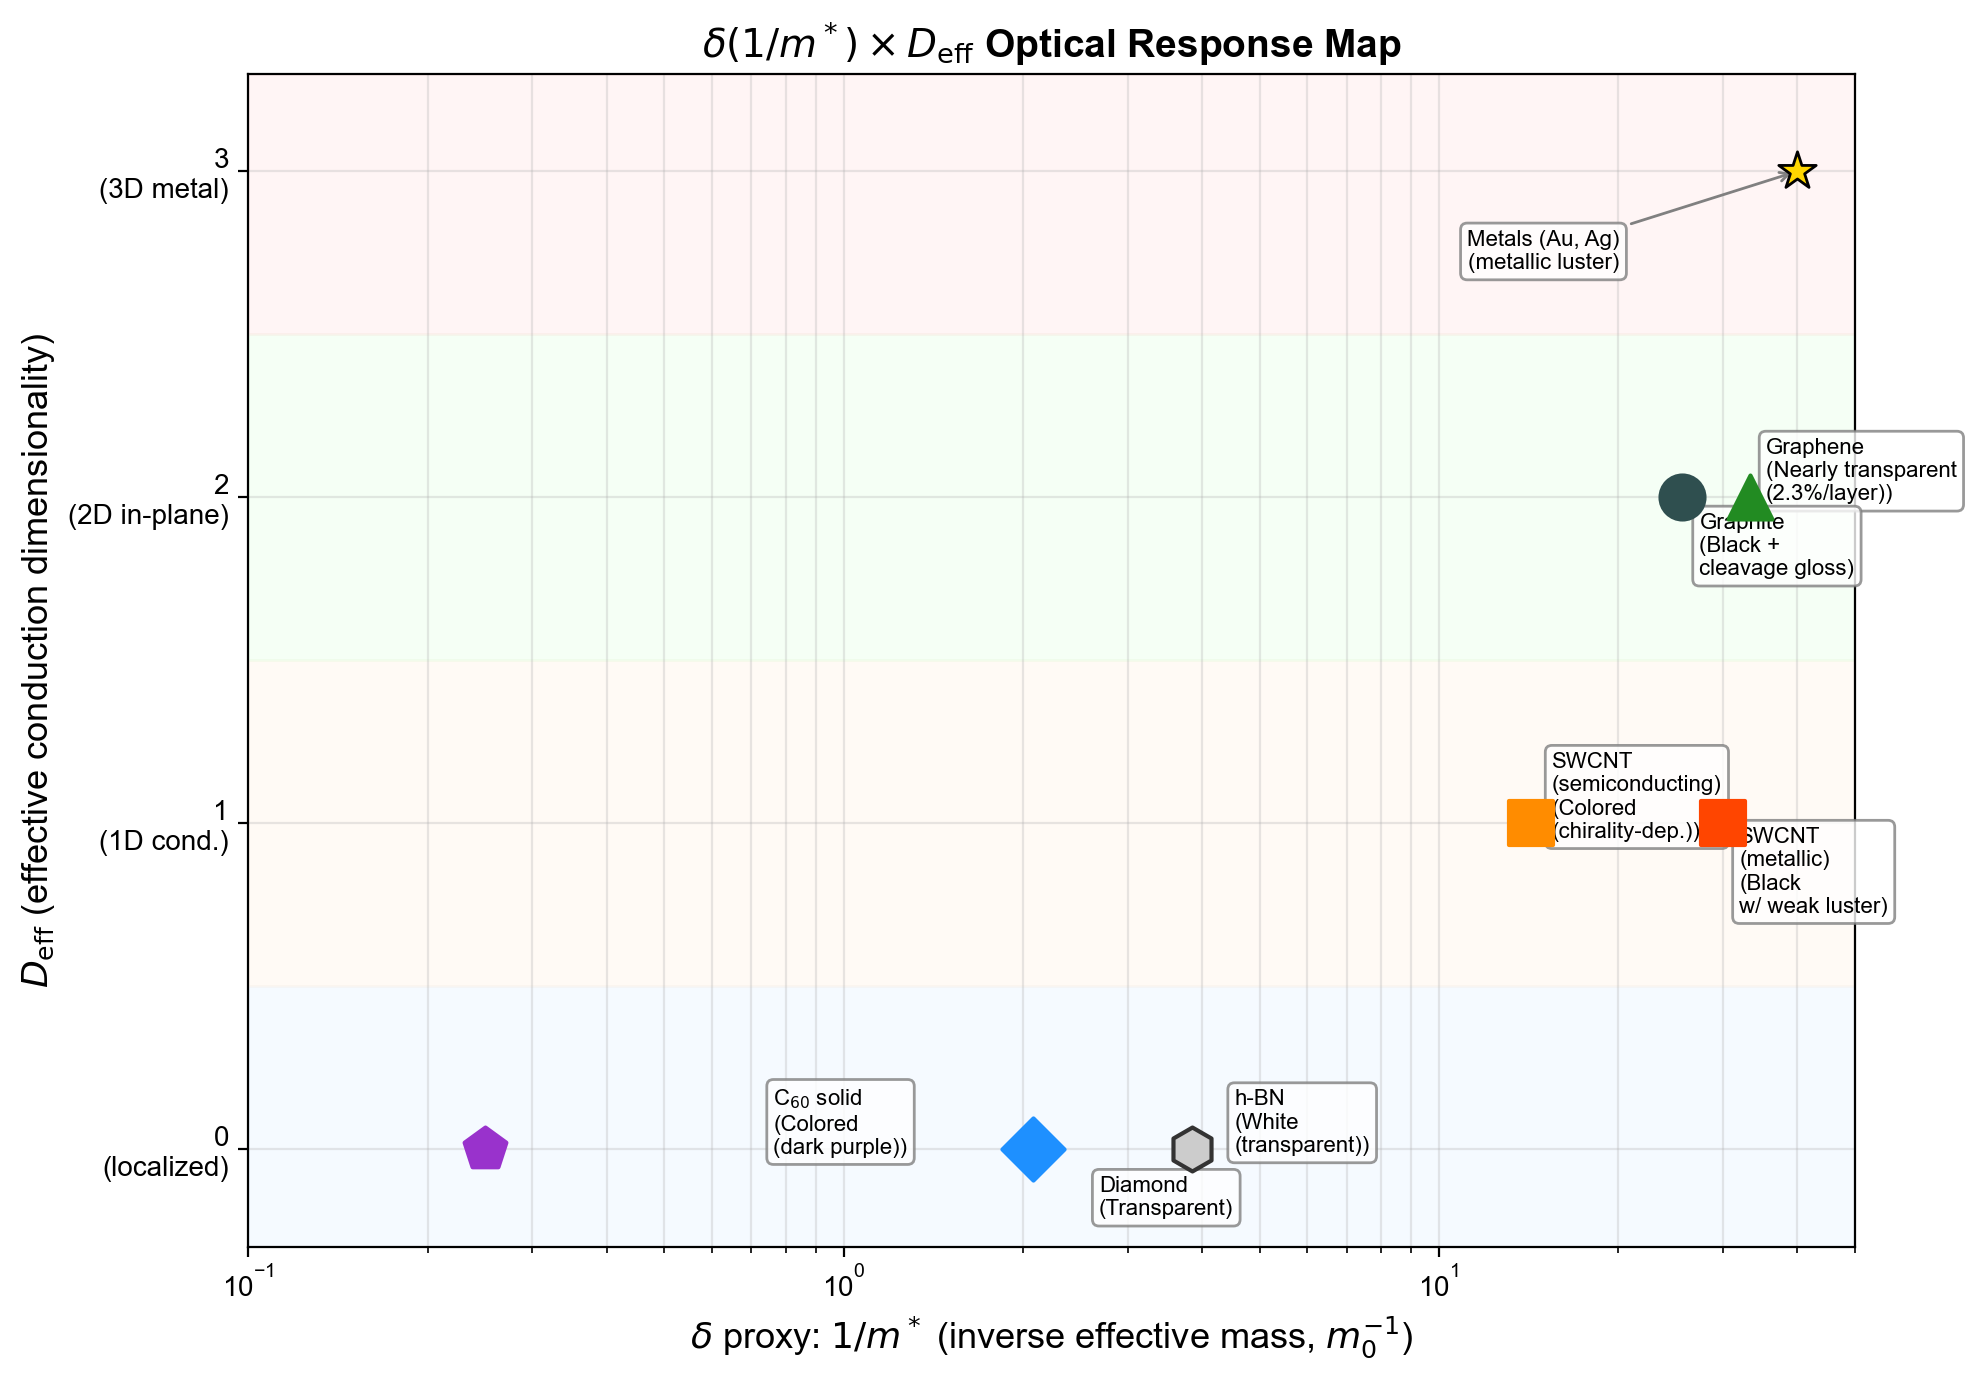
\includegraphics[width=\columnwidth]{fig3_invmass_deff_map}
  \caption{$\delta$（逆有効質量、対数スケール）と $D_\mathrm{eff}$
    のマップ。$\delta$ 軸に沿った物質の順序は
    図~\ref{fig:delta_map}と整合する。}
  \label{fig:invmass_map}
\end{figure}

\begin{figure}[t]
  
\includegraphics[width=\columnwidth]{fig2_delta_bandgap_correlation}
  \caption{公表データに基づく $\delta$（$\pi$ バンド幅）と
    バンドギャップ $E_g$ の関係（$r = -0.703$）。}
  \label{fig:delta_Eg}
\end{figure}

% =====================================================================
\section{考察}
\label{sec:discussion}
% =====================================================================

\subsection{コヒーレンス保存条件としての $\delta$}

本研究の出発点は「なぜ液体と金属の両方が光沢を示すのか？」
という問いであった。光沢は界面における光子の位相コヒーレンスの保存であり、
その条件は構成粒子の自由度（$\delta$）に帰着する。

ここで提示した固体での検証は、電子の非局在化~$\delta$ が
光学応答を支配する基本的変数であることを実証する。
Anderson 無秩序シミュレーション（第~\ref{sec:coherence}節）は
最初の直接的な数値的証拠を提供する。
高い $\delta \times D_\mathrm{eff}$ を持つ系は無秩序下でも
光学スペクトルを保存するのに対し、
低い $\delta \times D_\mathrm{eff}$ の系は急速にデコヒーレンスする。
この結果は、$\delta$---電子的であれ原子核的であれ---が
界面がコヒーレントな量子障壁として作用するか非コヒーレントな
量子障壁として作用するかを普遍的に決定するという、
より広範な仮説と整合する。

\subsection{Fresnel を超えて：類似の $\varepsilon$ が類似のグロスを
  意味しない理由}

Fresnel 方程式は、均一な $\varepsilon(\omega)$ で特徴づけられる
完全な無限半空間の反射率を予測する。現実には、
表面は決して完全ではない。原子スケールの無秩序、欠陥、
熱揺動が局所的な光学応答を変調する。
本研究の重要な知見は、\emph{無秩序ロバスト性}が
$\delta \times D_\mathrm{eff}$ に依存して系統的に変化する
ということである。

具体的には、C$_{60}$ とグラフェン/グラファイトは
類似したクリーン面反射率（$R_\mathrm{vis} \approx 0.40$ と
$0.35$）および同程度の $60^\circ$ グロス（394 対 366~GU）を持つ。
従来の Fresnel 光学は両者に同程度のグロスを予測するであろう。
しかし、Anderson 無秩序シミュレーションは、
同じ無秩序下で C$_{60}$ の光学応答がグラフェンの2倍の速さで
劣化することを示す。この差は $\delta \times D_\mathrm{eff}$
枠組みによって捉えられ、Fresnel 光学だけでは得られない予測を構成する。

\emph{物理的解釈}：拡張系（$D_\mathrm{eff} > 0$）では、
バンド分散が一種の「スペクトル慣性」を提供する---光学応答は
ブリルアンゾーンにわたる積分であり、局所的な摂動を平滑化する。
分子性系（$D_\mathrm{eff} = 0$）では、
応答は局所的無秩序に個別に敏感な離散エネルギー準位に依存する。

\subsubsection{1D鎖のパラドクス：IPR対スペクトル相関}

シミュレーションから明白なパラドクスが現れる。1D鎖は
無秩序下で\emph{最も速い} IPR成長（最も急速な波動関数の局在化）を
示すにもかかわらず、\emph{最も高い}スペクトル相関
（$W = 5$~eV で $r > 0.97$）を持つ。
これは矛盾ではない---IPRとスペクトル相関は
局在化の異なる側面を測定している。

IPRは\emph{個々の}固有状態の空間的広がりを探るものであり、
1Dでは Anderson 局在化が最も強く、固有状態は急速に局在する。
しかし、光学伝導率は\emph{全遷移にわたる和}
$\sigma(\omega) \propto \sum_{nm} |v_{nm}|^2
\delta(\omega - \omega_{nm})$ であり、そのスペクトル形状は
van~Hove 特異点（バンド端における状態結合密度の発散）に支配される。
これらの特異点は\emph{トポロジカルに保護}されている。
バンド構造のトポロジーに由来し、バンド端自体が破壊されない限り、
個々の状態が局在しても持続する。
したがって、1D鎖のスペクトル形状は波動関数が空間的に局在しても
ロバストである。

この区別は物理的に重要である。IPRはDC輸送（拡張状態を必要とする）
を支配し、スペクトル相関は\emph{光学}応答
（状態結合密度に依存する）を支配する。
ある物質は不良導体（局在状態、高IPR）でありながら、
光学反射率スペクトル（高スペクトル相関）を保持し得る。

\subsubsection{Anderson 無秩序モデルの範囲と限界}

重要な注意が必要である。ここで用いた Anderson オンサイト無秩序モデルは
\emph{バルク電子}コヒーレンスを探るものであり、
実際に鏡面グロスを支配する\emph{表面トポグラフィー的}粗さではない。
Beckmann--Spizzichino 枠組みでは、鏡面強度は
表面高さ分布（RMS粗さ $\sigma_h$、相関長 $\tau$）と
波長に依存する---いずれもバルクハミルトニアンでは捉えられない量である。

探索された無秩序の強さ（$W$ 最大5~eV）は広い範囲にわたることを
注記する。表面吸着物からの典型的なオンサイトエネルギー摂動は
0.3--1~eV、単一空孔からは1--2~eV、置換不純物からは2--4~eVである。
したがって $W = 0.5$--$2$~eV は現実的な表面近傍の摂動を表し、
$W = 5$~eV は極端なストレステストである。
重要なことに、系間の\emph{順位}（1D鎖 $>$ グラフェン $>$ C$_{60}$）は
全ての $W$ 値にわたって一貫しており、
相対的なコヒーレンス保存がバンド構造の頑健な性質であり、
無秩序の強さのアーティファクトではないことを示す。

本モデルは関連するが異なる問いに取り組む。\emph{平坦な}界面が
与えられたとき、物質の誘電応答 $\varepsilon(\omega)$ は
原子スケールの組成的または構造的無秩序に対してどの程度ロバストか？
バルク無秩序を表面グロスに結びつける物理的議論は以下の通りである。
(i)~表面原子はバルク原子と異なる局所環境を経験し
（配位数の低下、再構成、吸着物）、有効なオンサイトエネルギー摂動を生む。
(ii)~$\varepsilon(\omega)$ がそのような摂動にロバストであれば、
表面近傍の誘電プロファイルは均一に保たれ、Fresnel 反射が保存される。
(iii)~$\varepsilon(\omega)$ が脆弱であれば、
表面近傍領域が光学的に不均一となり、
原子的に平坦な表面上でさえ光を拡散散乱する。

この推論の連鎖は妥当であるが厳密に導出されたものではない。
完全な処理には Anderson 無秩序モデルを
表面散乱枠組み（例えば表面粗さの Rayleigh--Rice 摂動論、
あるいは巨視的トポグラフィーのマイクロファセットモデル）と
結合する必要がある。$\delta \times D_\mathrm{eff}$ を
確立されたグロスモデルに入る粗さパラメータ
（$\sigma_h$, $\tau$）に接続することを、
将来の研究の具体的目標として提案する。

\subsection{$D_\mathrm{eff}$ と伝導率テンソルの異方性}

$D_\mathrm{eff}$ は、測定または計算された伝導率テンソルの異方性と
比較することで独立に検証できる。グラファイトでは、
面内と面外の伝導率が $\sim$$10^3$ 倍異なる
（$\sigma_\parallel / \sigma_\perp \approx
10^3$）~\cite{Spain1981}。これは面内 $\pi$ バンド分散の
弱い層間ホッピング（$\gamma_1 \approx 0.4$~eV $\ll$
$W_\pi \approx 9$~eV）に対する優位性を反映する。
この極端な異方性はまさに $D_\mathrm{eff} = 2$ が符号化するものである。
速度テンソルの有効ランクは、光学応答が2つの空間方向に限定されている
という事実を捉える。ダイヤモンドでは
$D_\mathrm{eff}^\mathrm{all} = 3$ が等方的な sp$^3$ ネットワークを反映し、
観測される等方的伝導率および屈折率と整合する。
C$_{60}$ 固体では $D_\mathrm{eff} = 0$ が分子性を反映する。
3D fcc格子に結晶化するにもかかわらず、
狭い分子間バンド（$W \approx 0.5$~eV）は
光学応答において無視できる方向異方性しか生じない。

$D_\mathrm{eff}$ をテンソル的光学伝導率データベース
（例えば大規模 Wannier 計算）と系統的に比較することは、
厳密で独立した検証を提供し得るものであり、
将来の研究目標として提案する。

\subsection{$\delta$、$E_g$、$D_\mathrm{eff}$ の役割}

本研究の貢献は、$E_g$ と並ぶ第二の分類軸として
$D_\mathrm{eff}$ を導入したことにある：
\begin{itemize}
  \item $E_g$ は光学応答が\emph{どのエネルギーで}生じるかを決定する。
  \item $D_\mathrm{eff}$ は応答が\emph{何方向の空間方向に}
    強いかを決定し、$E_g$ だけでは区別できない縮退を解消する
    （例：$E_g \approx 0$ におけるグラファイト対金属）。
  \item 粒子の自由度（$\delta$）の概念が $D_\mathrm{eff}$ の
    導入を動機づけた。$\delta$ 自体は本研究では分類変数として
    使用しない。その独立検証---特に $E_g$ が定義困難な
    液体系や界面系への拡張を通じて---は、
    将来の研究の自然な目標である。
\end{itemize}

\subsection{既存理論との関係}

\begin{table}[h]
\caption{$\delta \times D_\mathrm{eff}$ 枠組みと既存理論の関係。}
\label{tab:existing}
\begin{ruledtabular}
\begin{tabular}{ll}
  Existing theory & Relation to present framework \\
  \hline
  Drude model & Special case: $D_\mathrm{eff} = 3$, $\delta$ high \\
  Band theory & $E_g$ is one axis; $D_\mathrm{eff}$ adds the second \\
  Crystal-field theory & $10Dq \approx$ local modulation of $\delta$ \\
  Fresnel optics & Presupposes uniform $\varepsilon(\omega)$; \\
   & this uniformity itself depends on $\delta$ \\
  Anderson localization & Disorder-induced $\delta$ reduction; \\
   & directly tested in this work \\
\end{tabular}
\end{ruledtabular}
\end{table}

\subsection{h-BN と副格子対称性の破れ}
\label{sec:hBN_discussion}

グラファイト（黒色）と h-BN（白色）の劇的な光学的コントラストは、
従来 B--N の電気陰性度差による副格子対称性の破れに帰せられてきた。
本枠組みでは、この対称性の破れは直接的に翻訳される。
交互オンサイトポテンシャル~$\Delta$ が $\pi$ 電子を
窒素サイトに局在化させ、$\delta$ を\emph{低下させる}。
定量的には、副格子ポテンシャル~$\Delta$ を持つ
ハニカム格子の tight-binding モデルは $E_g = 2\Delta$ を与え、
光学遷移に利用可能な有効バンド幅を低下させる。
対称性の破れ（バンド理論）と $\delta$ の低下（本枠組み）という
2つの記述は、二部格子に対して数学的に等価であり、
$\delta$ の言語が標準的な固体物理の描像と矛盾せず
整合していることを確認する。

\subsection{先行研究}

我々の知る限り、以下を行った先行出版物は存在しない：
\begin{enumerate}
  \item バンドギャップと有効伝導次元数を用いて巨視的光学応答を
    分類する明示的な決定木を構築すること。
  \item $D_\mathrm{eff}$ を結晶学的次元数と異なる
    形式的分類変数として定義すること。
  \item Tight-binding パラメータから産業標準グロス単位 [GU] への
    予測連鎖を確立すること。
  \item Anderson 無秩序シミュレーションを通じてコヒーレンス保存仮説を
    数値的に検証すること。
  \item 複数の非局在化代理指標を単一の包括的指数 $\delta$ の下に
    統一し、その相互整合性を検証すること。
\end{enumerate}

最も近い関連研究は Shi and Yao \textit{et al.}（Carbon, 2020）であり、
密度と結合角を用いて炭素同素体を金属、半導体、絶縁体に分類した。
しかし、その枠組みは\emph{光学的外観}ではなく\emph{電子相}を対象としており、
次元数変数を欠いている。

\subsection{Wannier スプレッドによる第一原理的確認}
\label{sec:wannier_confirmation}

主たる分類（Secs.~\ref{sec:results}--\ref{sec:disorder}）は
文献由来の代理指標とタイトバインディングモデルに基づく。
これらは $\delta$ の存在を支持するが、第一原理レベルでの直接計算ではない。
\emph{独立な確認}として、バルクダイヤモンドおよびグラファイトに対して
DFT (PBE) + Wannier90 計算を実行し、最大局在化 Wannier 関数（MLWF）の
スプレッド~$\Omega$~\cite{Marzari1997}を求めた。
$\Omega$ は固体中の各電子の空間的広がりを直接測定する量である。
この確認は分類分析とは独立であり、代理指標で確立した $\delta$ 順序が
第一原理レベルで再現されることを検証する目的で行った。

結果は明確である：$\Omega/\mathrm{WF} = 0.95$~\AA$^2$（ダイヤモンド）
対 $6.38$~\AA$^2$（グラファイト）、6.7倍の比である。
さらに、グラファイトの 8 つの Wannier 関数は 6 つの
$\sigma$ 型（5.5--6.3~\AA$^2$）と 2 つの $\pi$ 型
（7.3--8.2~\AA$^2$）に分解され、$\pi$ 電子の非局在化が
グラファイトの金属的光学応答の微視的起源であることが確認された。

計算をシリコン（$\Omega/\mathrm{WF} = 3.05$~\AA$^2$）および
ゲルマニウム（$2.28$~\AA$^2$）に拡張すると、$\Omega$ 単独では
異なる元素間の屈折率を予測できないことが明らかになる：
$\Omega(\mathrm{Ge}) < \Omega(\mathrm{Si})$ であるのに
$n(\mathrm{Ge}) > n(\mathrm{Si})$。これは Penn モデル~\cite{Penn1962}
と整合的であり、誘電率は電子非局在化、原子分極率、バンドギャップの
3つの独立な因子に依存する。単一元素（炭素同素体）内では
後者の2つが構造と共変するため $\delta$ 単独で十分であり、
これが本研究の分類の成功を説明する。

\subsection{光学 sum rule と $\delta$ の数学的基盤}
\label{sec:sum_rule}

最近、Cardenas-Castillo \textit{et al.}~\cite{CardenasCastillo2024} は、
Wannier スプレッドのゲージ不変部分~$\Omega_I$ が
光学吸収の周波数重み付き積分に等しいことを証明した：
\begin{equation}
  \Omega_I = \frac{\hbar^2 e^2}{2\pi m^2}
  \int_0^\infty \frac{\mathrm{Im}[\varepsilon(\omega)]}{\omega}\,d\omega.
  \label{eq:sum_rule}
\end{equation}
量子幾何に根ざすこの恒等式~\cite{RhimKim2025}は、
電子非局在化と光学応答の間に厳密な数学的接続を確立する：
$\delta$ と光学吸収は単に相関しているのではなく、
sum rule により関係づけられている。

$\delta \times D_\mathrm{eff}$ による炭素同素体の分類は、
この恒等式の順方向の利用として理解できる：
$\Omega$ を測定スペクトルからの抽出ではなく、光学カテゴリの
予測子として用いる。sum rule は $\delta$ の適用範囲をも明確にする：
$\delta$ は全周波数にわたる\emph{積分}光学吸収を支配するのであって、
特定の波長での応答ではない。
単一元素内では $\varepsilon_2(\omega)$ のスペクトル形状が
同素体間で穏やかにしか変化しないため、
積分量の序列が各周波数での序列を近似する---
これが 6/7 の分類成功の理由である。
異なる元素間ではスペクトル形状が大きく異なり、
$\delta$ 単独では特定波長の $n$ を予測しなくなる。

Moss~\cite{Moss1950} および Ravindra~\cite{Ravindra2007}
の経験的 $n$--$E_g$ 関係は相補的と見なせる：
$\delta$ が含まない $E_g$ 依存性を捉えている。
Penn モデル~\cite{Penn1962} とともに、これらは
$\delta$ が非局在化因子として独自の位置を占める
理論的な地形を確立する。

\subsection{限界}

\begin{enumerate}
  \item 検証は7物質（5種の炭素同素体 + h-BN + 金属基準）に限定される。
    この制限は\emph{意図的}である。単一元素を使用することで
    元素組成を交絡因子から排除し、$\delta$--$D_\mathrm{eff}$ 仮説の
    最もクリーンな検証を提供する。
    元素をまたいだ検証（遷移金属、極性誘電体、擬1D導体、層状酸化物）は
    自然な次のステップである。
    姉妹論文~\cite{SentoOpticsPaper2}は $\delta$ 枠組みを
    表面張力の文脈で11種の金属元素に拡張する。
  \item $\delta$ の操作的定義は一意ではない。しかし、
    3つの独立した代理指標間の一致がその存在に対する
    経験的裏付けを提供する。
  \item グラフェンからグラファイトへのクロスオーバーには
    厚さ~$N$ が追加パラメータとして必要である
    （Beer--Lambert 領域）。
  \item コヒーレンス保存テストは有限スーパーセル
    （グラフェン200サイト、1D鎖200サイト、C$_{60}$ 60サイト）
    を使用しており、定量的な局在長にはより大きな系が必要である。
  \item 有効グロスモデル（式~\ref{eq:eff_gloss}）は単純な
    $\mathrm{corr}^2$ スケーリングを仮定している。
    より厳密な処理には完全な表面散乱理論
    （例えば Beckmann--Spizzichino）が必要である。
  \item ダイヤモンドの可視域反射率（$R_\mathrm{vis} = 0.17$）には
    シザーズ補正と実験的 $\varepsilon_\infty = 5.7$~\cite{Palik1998}
    が入力として必要であり、完全な\emph{ab initio}予測には
    より完全な基底関数セットまたはGW補正が必要である。
  \item 励起子効果と局所場効果は、C$_{60}$ と h-BN では大きいが、
    ここで用いた独立粒子近似（IPA）では無視されている。
    GW/BSE計算は $\varepsilon(\omega)$ の定量的精度を向上させるであろう。
  \item 可視域平均は平坦なスペクトル重みを使用する。
    CIE明所視感度重み（ガウス近似、$555$~nmにピーク）を用いると
    $R_\mathrm{vis}$ の変化は$<$12\%であり全体的順位は保存される
    （ダイヤモンド $<$ グラフェン $<$ 1D鎖）。
    C$_{60}$/1D の相対的順序は重み付けの選択に敏感である。
\end{enumerate}

\subsection{展望}

\begin{itemize}
  \item \textbf{グロス予測の実験的検証}：グラファイトと
    C$_{60}$ 単結晶の $60^\circ$ グロスを測定し、
    予測された有効グロス値（表~\ref{tab:eff_gloss}）と比較する。
  \item \textbf{液体}：原子核の非局在化 $\delta_\mathrm{nuc}$ と
    界面自己平滑化におけるその役割。
    ガリウムの固体-液体反射率ジャンプ（50\% $\to$ 90\%）は
    直接的なテストケースである。
  \item \textbf{界面と触媒}：ヘテロ接合における $\delta$ の不連続性が
    電荷移動速度を支配するかどうか。
    触媒活性のdバンド中心理論との関連。
  \item \textbf{$\Omega$ からの前方予測}：本研究で報告した
    Wannier スプレッド計算（第~\ref{sec:wannier_confirmation}~節）は
    $\delta$ の序列を第一原理レベルで確認した。
    次のステップは Wannier 補間光学伝導率（postw90）により
    $\varepsilon_2(\omega)$ を計算し、$\Omega$ が積分光学吸収を
    予測すること（式~\ref{eq:sum_rule}）を実証する---
    $\Omega \to \varepsilon(\omega)$ の因果連鎖を
    単一の計算フレームワーク内で閉じることである。
  \item \textbf{$\delta$ の精密な定義}：本研究では $\delta$ は
    代理指標の整合性と Wannier スプレッドの序列に支持された
    現象論的変数にとどまる。$\Omega$ に基づく $\delta$ の
    厳密な定義と、原子核の自由度との関係は、
    将来の研究（Paper~III）に委ねる。
  \item \textbf{逆設計}：目標の光学応答が与えられたとき、
    $\delta \times D_\mathrm{eff}$ を反転して候補構造を
    同定する。
  \item \textbf{元素をまたいだ検証}：遷移金属酸化物、
    有機半導体、ペロブスカイト。
\end{itemize}

% =====================================================================
\section{結論}
\label{sec:conclusion}
% =====================================================================

光沢とは界面における光子の位相コヒーレンスの保存である。
我々は、その微視的条件が構成粒子の自由度に帰着し、
非局在化指数~$\delta$ によって定量化されることを提案する。

概念実証として、二変数の現象論的枠組み
（$\delta_\mathrm{elec}$, $D_\mathrm{eff}$）を構築し、
5種の炭素同素体とh-BN対照系で検証した。
$E_g$ と $D_\mathrm{eff}$ に基づく決定木は、
7物質中6物質を正しい光学応答カテゴリー
（透明、有色、黒色、光沢）に分類する。
唯一の例外---単層グラフェン---は第三のパラメータとして
層数~$N$ を必要とする。

分類を超えて、微視的パラメータ（ホッピング積分、軌道対称性）から
産業標準単位 [GU] での巨視的グロスへの完全な予測連鎖を確立した。
Anderson 無秩序シミュレーションはコヒーレンス保存仮説の
最初の数値的証拠を提供する。
高い $\delta \times D_\mathrm{eff}$ を持つ系は
原子スケールの無秩序下でも光学応答を維持するのに対し、
分子性系（$D_\mathrm{eff} = 0$）は急速にデコヒーレンスする。
これにより Fresnel 光学だけでは得られない予測が得られる。
クリーン面の反射率が類似した物質であっても、
無秩序ロバスト性の違いにより非常に異なる有効グロスを示し得る。

本枠組みはバンドギャップ理論を置き換えるものではなく、
$D_\mathrm{eff}$ を第二の分類軸として、
無秩序ロバスト性を第三の予測次元として追加することで
それを拡張する。
$E_g$ は応答が\emph{どのエネルギーで}生じるかを決定し、
$D_\mathrm{eff}$ はその\emph{方向性}を決定し、
$\delta$ はその\emph{ロバスト性}を決定する。
$D_\mathrm{eff}$ の導入を動機づけた粒子の自由度（$\delta$）の概念は、
独立した検証が残されている。$E_g$ が定義困難であるが
$\delta$ が依然として適用可能であり得る
液体系、界面系、および元素をまたいだ系への拡張を、
将来の研究目標として提案する。
\paragraph{展望。}
$\delta$ は特定のプローブではなく界面における粒子の自由度を
特徴づけるため、表面張力や電気伝導率など他の界面支配的特性にも
関連し得る。Wannier スプレッド~$\Omega$---厳密に定義された
第一原理量---は $\delta$ の精密な定義の自然な候補であり、
結晶系のみならず液体を含む無秩序系にも適用可能である。

\begin{acknowledgments}
本研究の着想は、銭湯（\textit{sent\=o}）において
水面の光沢を観察したことに端を発する。
\end{acknowledgments}

\section*{データおよびコードの利用可能性}

全てのシミュレーションコード（\texttt{delocalization\_optics\_v2.py}）、
tight-binding パラメータ、計算された $\varepsilon(\omega)$ スペクトル、
および図生成スクリプトは以下で公開されている：
\url{https://github.com/miyauchikazuyoshi/sento-optics}。

\section*{AI支援ツールの使用}

概念的枠組み---粒子の自由度（$\delta$）が界面における光子の
コヒーレンス保存を支配するという仮説、$\delta$ と $D_\mathrm{eff}$
の定義、および決定木による分類---は著者が独自に構想したものである。

実験設計、文献データ収集、統計的検証、tight-binding シミュレーションコード、
および原稿執筆は、大規模言語モデル
（Claude, Anthropic; ChatGPT, OpenAI; Gemini, Google）の
実質的な支援を受けて実施した。具体的には：

\begin{itemize}
  \item \textbf{データ収集}：$\pi$ バンド幅、有効質量、バンドギャップ、
    光学特性の公表値は、AI支援により文献から収集した。
    全ての値は著者が一次文献と照合して確認した。
  \item \textbf{シミュレーション}：Tight-binding 概念実証コード
    （\texttt{delocalization\_optics\_v2.py}）はAI支援により開発した。
    コードとその出力は著者が確認・検証した。
  \item \textbf{統計解析}：相関分析および分類テストは
    AI支援により実施し、著者が独立に検証した。
  \item \textbf{原稿}：英語草稿は、著者の日本語ノートおよび
    構造的アウトラインに基づき、AI支援により作成した。
  \item \textbf{査読シミュレーション}：投稿前の査読フィードバックを
    複数のAIシステムに依頼し、潜在的な弱点を特定して
    原稿を強化した。
\end{itemize}

\noindent データ検証用コードおよび研究ノートは
\url{https://github.com/miyauchikazuyoshi/sento-optics}
にて公開している。

\noindent 著者は、本研究で提示された科学的内容、解釈、
および結論に対する全責任を負う。

\bibliography{references}

\end{document}
